\section{Appendix B: Non-Averaged Curves}

In this section we provide additional learning curves, variance curves, and gap curves. In contrast to the curves presented in the paper's body, these curves were not averaged over 64 different experiments. Rather, they are obtained from a single experiment. Note, however, that these curves still do report average performance over 64 held-out test environments. This is presented to show that the curves generated from individual experiments are largely reasonable. Further, for these experiments we utilized different test environment seeds than those utilized in the paper's body, to show that we are not over-fitting to those particular seeds.

The results are consistent with those presented in the paper. 

\begin{figure}[H]
\begin{center}
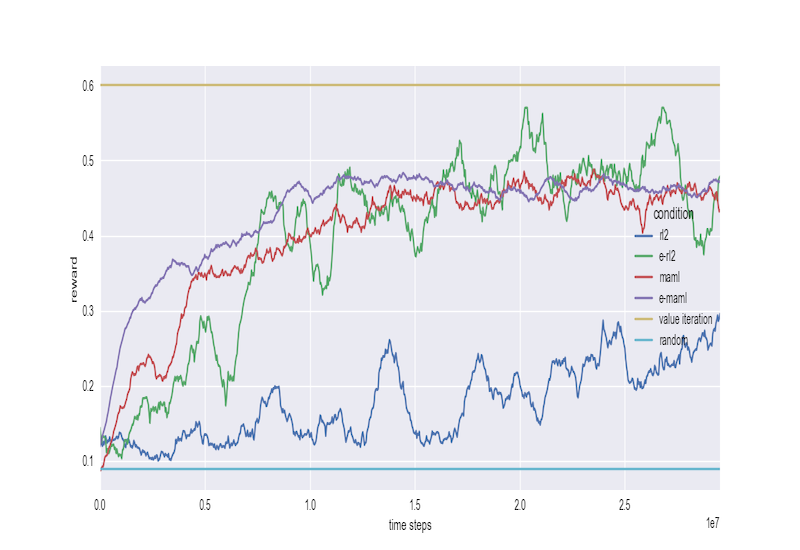
\includegraphics[scale=0.335]{bradly_curves/64testgrid0_scaled.png}%
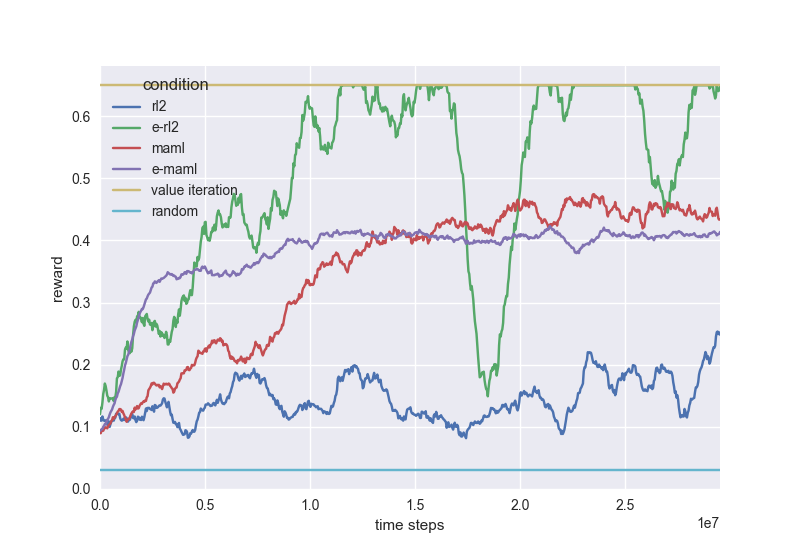
\includegraphics[scale=0.335]{bradly_curves/64testgrid1.png} \\
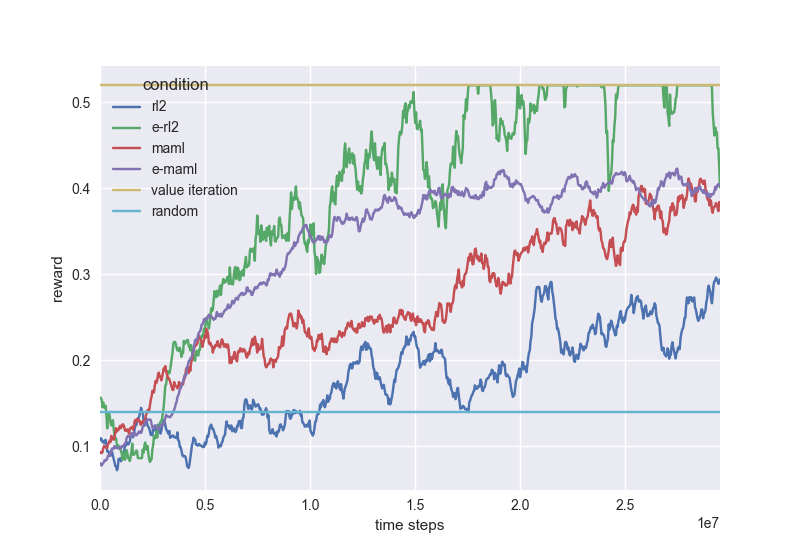
\includegraphics[scale=0.335]{bradly_curves/64testgrid2.png}%
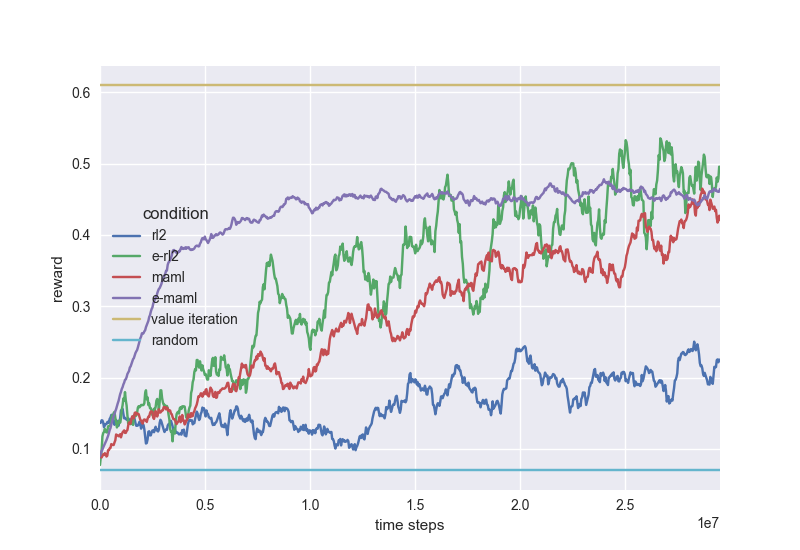
\includegraphics[scale=0.335]{bradly_curves/64testgrid3.png}
\end{center}
\caption{Learning curves for 4 different seeds of test environments.}
\label{fig:appendix-learning-curves-0}
\end{figure} 

\begin{figure}[H]
\begin{center}
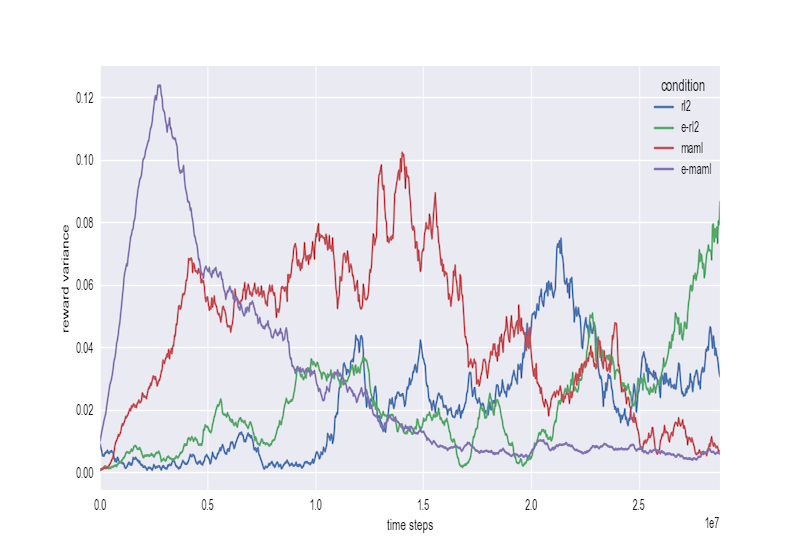
\includegraphics[scale=0.335]{bradly_curves/64testgridvar0_scaled.png}%
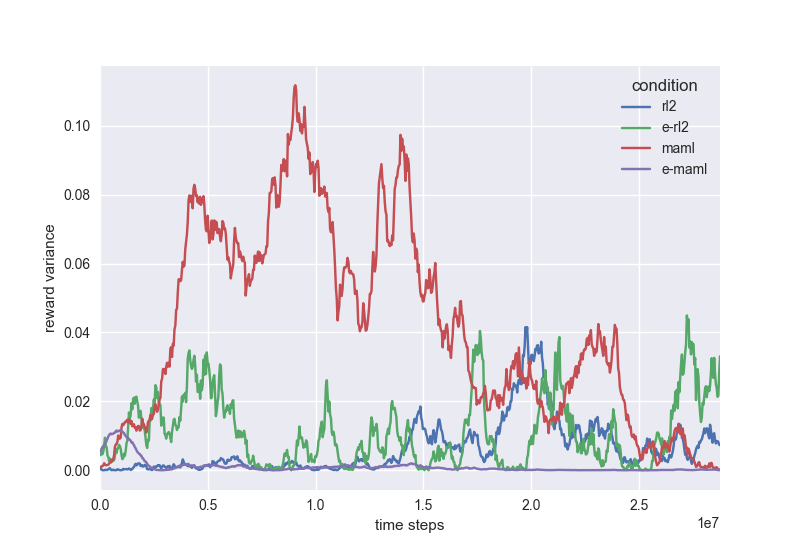
\includegraphics[scale=0.335]{bradly_curves/64testgridvar1.png} \\
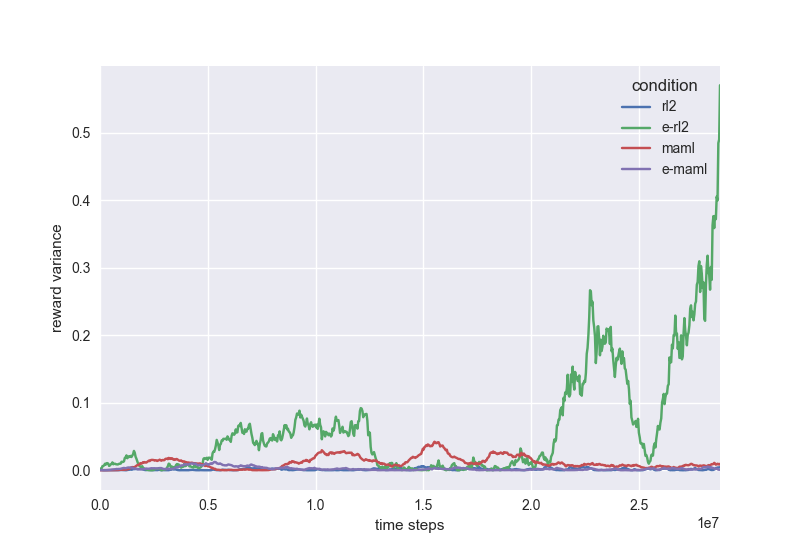
\includegraphics[scale=0.335]{bradly_curves/64testgridvar2.png}%
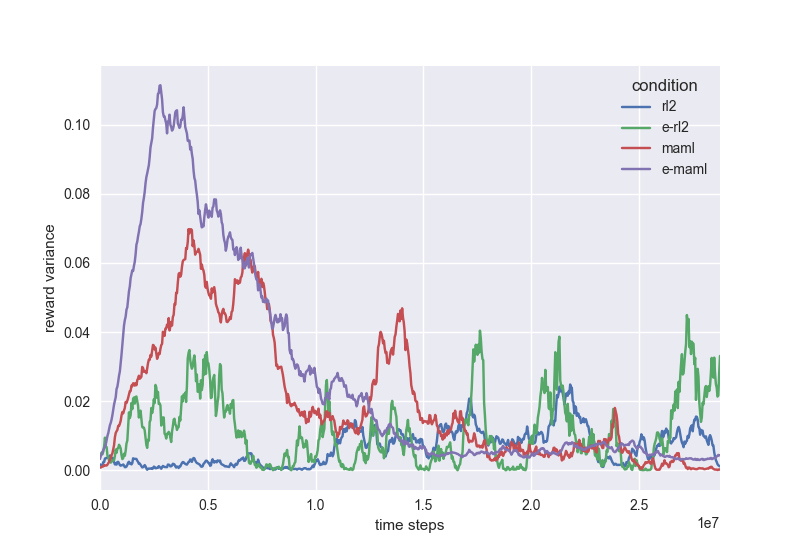
\includegraphics[scale=0.335]{bradly_curves/64testgridvar3.png}
\end{center}
\caption{Variance curves for 4 different seeds of test environments.}
\label{fig:apprendix-variance-curves-1}
\end{figure} 

\begin{figure}[H]
\begin{center}
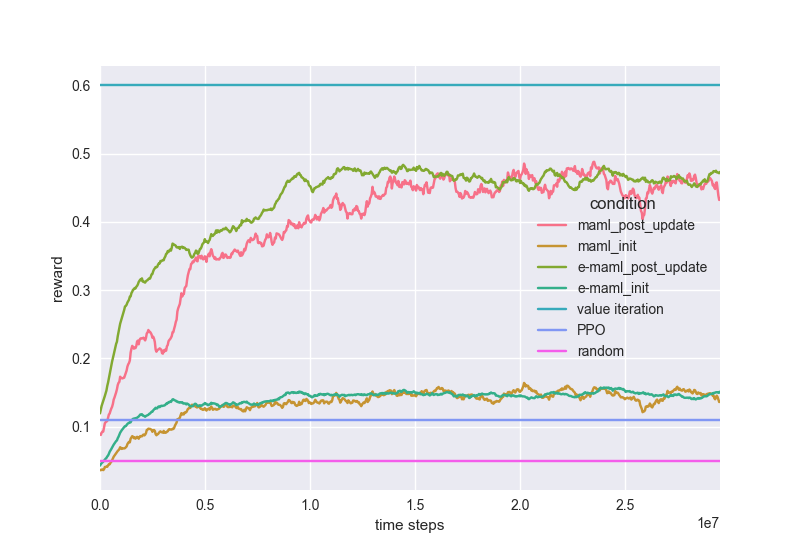
\includegraphics[scale=0.335]{bradly_curves/gap_grids_maml_0.png}%
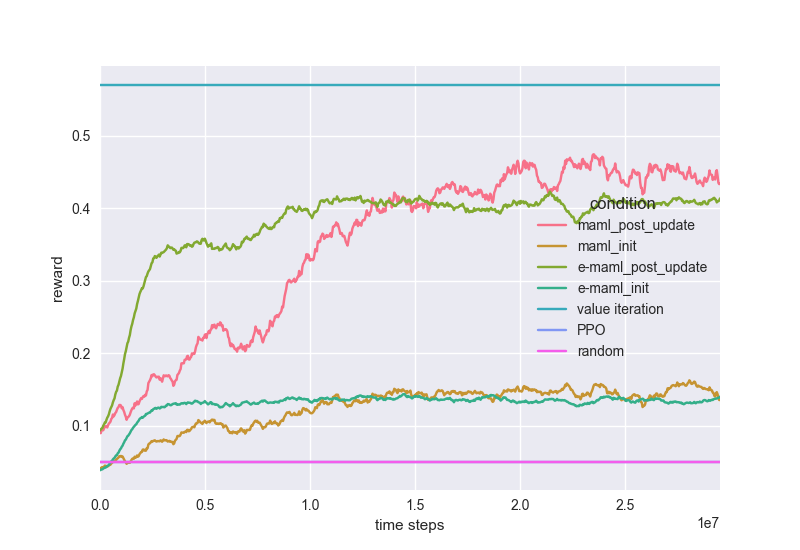
\includegraphics[scale=0.335]{bradly_curves/gap_grids_maml_1.png} \\
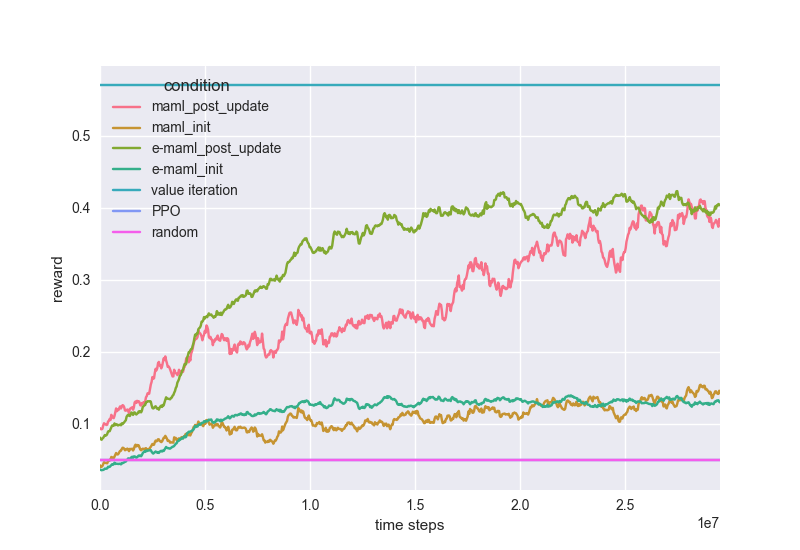
\includegraphics[scale=0.335]{bradly_curves/gap_grids_maml_3.png}%
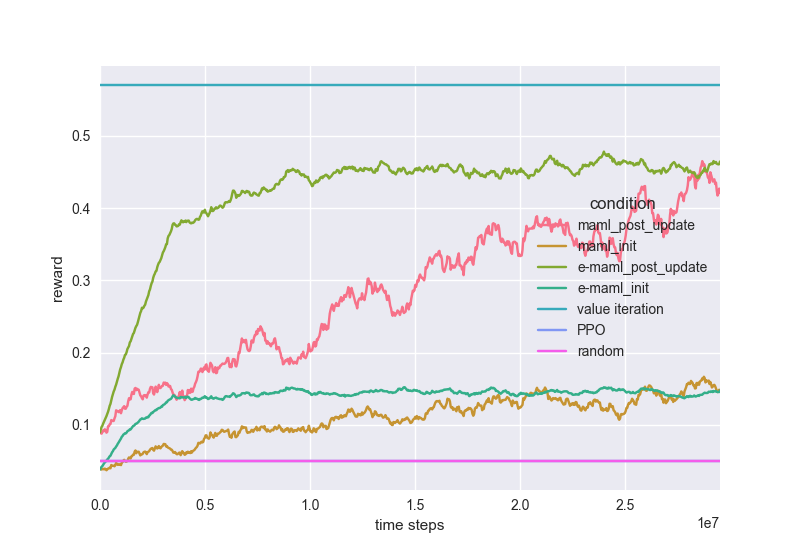
\includegraphics[scale=0.335]{bradly_curves/gap_grids_maml_4.png}
\end{center}
\caption{First-update-performance-gap curves for 4 different seeds of test environments. Results for MAML and E-MAML}
\label{fig:appendix-gap-curves-0}
\end{figure} 

\begin{figure}[H]
\begin{center}
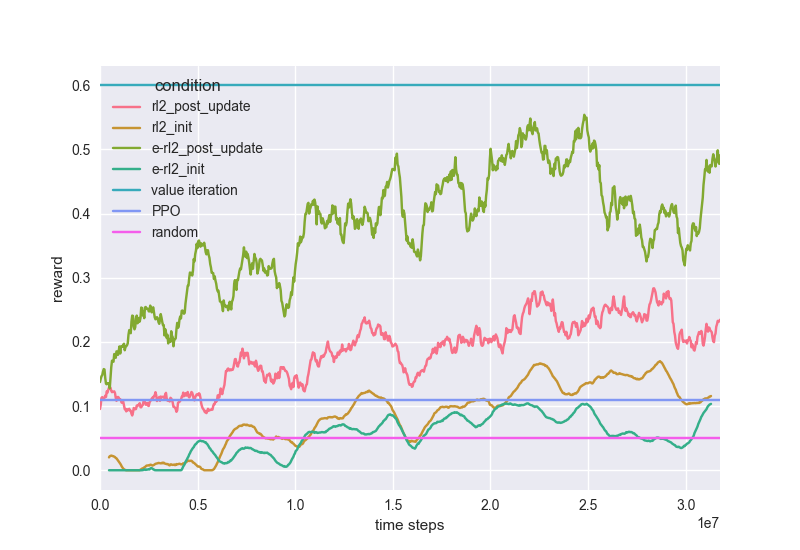
\includegraphics[scale=0.335]{bradly_curves/gap_grids_rl2_0.png}%
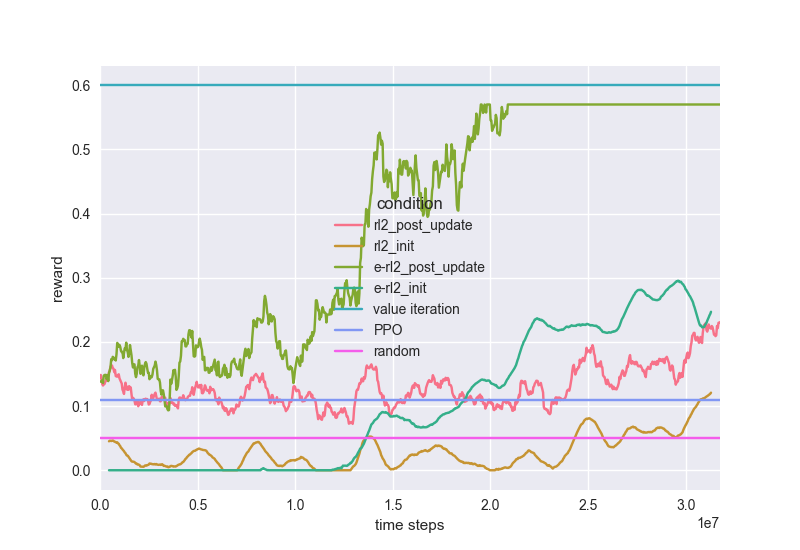
\includegraphics[scale=0.335]{bradly_curves/gap_grids_rl2_1.png} \\
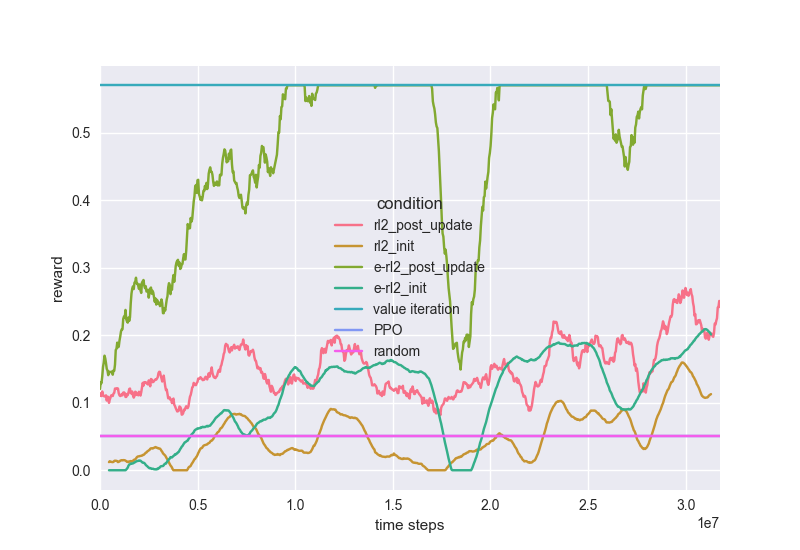
\includegraphics[scale=0.335]{bradly_curves/gap_grids_rl2_2.png}%
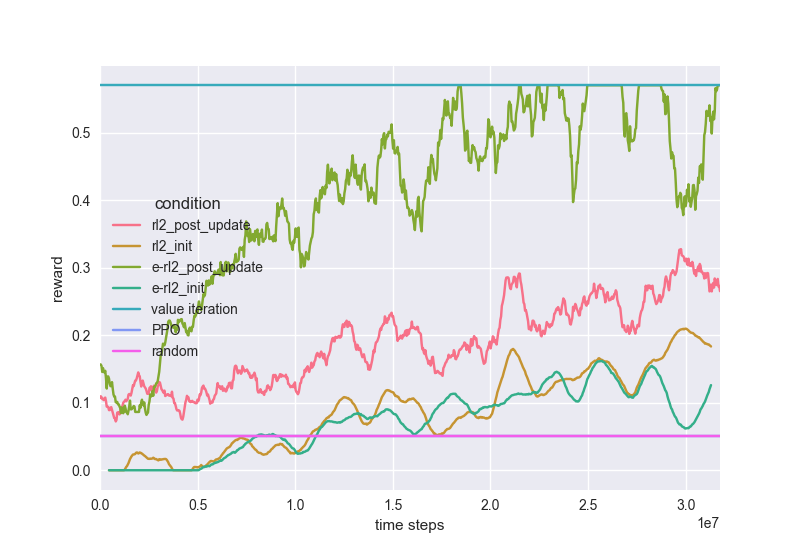
\includegraphics[scale=0.335]{bradly_curves/gap_grids_rl2_3.png}
\end{center}
\caption{First-update-performance-gap curves for 4 different seeds of test environments. Results for E-$\text{RL}^2$ and $\text{RL}^2$.}
\label{fig:appendix-gap-curves-1}
\end{figure}